\documentclass[11pt]{beamer}
\setbeamertemplate{navigation symbols}{}
 \setbeamercovered{transparent}
\usepackage{listings}
%\usetheme{Copenhagen}
\usetheme{Singapore}
%\usetheme{Madrid}
%\usetheme{Hannover}
%\usetheme{boxes}
%\usetheme{Boadilla}
\usefonttheme[onlymath]{serif}
\usecolortheme{beaver}
\usepackage{textpos}
\usepackage{fancyvrb}
\usepackage{xcolor}
\usepackage{multicol}
\usepackage{lipsum}
\parskip 1ex

\newcommand\FontAcolumn{\fontsize{6}{7.2}\selectfont}
\newcommand\FontBcolumn{\fontsize{8}{7.2}\selectfont}
\newcommand\FontCcolumn{\fontsize{10}{7.2}\selectfont}
\newcommand\FontDcolumn{\fontsize{11}{7.2}\selectfont}

\definecolor{gray97}{gray}{.97}
\definecolor{gray75}{gray}{.75}
\definecolor{gray75}{gray}{.45}

\lstdefinestyle{Fortran}{language=[90]Fortran}

\newcommand\FortranStyle
{
\lstset{
frame=Ltb,
framerule=0pt,
columns=fullflexible,
aboveskip=0.5cm,
framextopmargin=3pt,
framexbottommargin=3pt,
framexleftmargin=0.4cm,
framesep=0pt,
rulesep=.4pt,
backgroundcolor=\color{gray97},
rulesepcolor=\color{black},
stringstyle=\ttfamily,
showstringspaces=false,
basicstyle=\ttfamily,
commentstyle=\color{green},
keywordstyle=\color{red},
numbers=left,
numbersep=15pt,
numberstyle=\tiny,
numberfirstline=false,
breaklines=true,
 tabsize=2,
 extendedchars=true,
keepspaces,
}
}

\newcommand\FortranStyleA
{
\lstset{
frame=Ltb,
framerule=0pt,
columns=fullflexible,
aboveskip=0.5cm,
framextopmargin=3pt,
framexbottommargin=3pt,
framexleftmargin=0.4cm,
framesep=0pt,
rulesep=.4pt,
backgroundcolor=\color{gray97},
rulesepcolor=\color{black},
stringstyle=\ttfamily,
showstringspaces=false,
basicstyle=\ttfamily,
commentstyle=\color{green},
keywordstyle=\color{red},
numbersep=15pt,
numberstyle=\tiny,
numberfirstline=false,
breaklines=true,
 tabsize=2,
 extendedchars=true,
keepspaces,
}
}

\newcommand\tab[1][1cm]{\hspace*{#1}}
\newcommand{\light}[1]{\textcolor{lightgray}{#1}}
    
\def\signed #1{{\leavevmode\unskip\nobreak\hfil\penalty50\hskip2em
  \hbox{}\nobreak\hfil(#1)%
  \parfillskip=0pt \finalhyphendemerits=0 \endgraf}}

\newsavebox\mybox
\newenvironment{aquote}[1]
  {\savebox\mybox{#1}\begin{quote}}
  {\signed{\usebox\mybox}\end{quote}}


% items enclosed in square brackets are optional; explanation below
\title{Object Oriented Fortran}
\subtitle{An Overview}
\author{Carlos Cruz}
\institute{
  NASA GSFC Code 606 (ASTG)\\
  Greenbelt, Maryland 20771\\[1ex]
  \texttt{carlos.a.cruz@nasa.gov}
}
\date{October 25, 2018}

\begin{document}

% --- Title page ---
\begin{frame}[plain]
  \titlepage
\end{frame}

\logo{%
  
\includegraphics[width=1cm,height=1cm,keepaspectratio]{../../shared/nasa-ball.png}%
  \hspace{\dimexpr\paperwidth-2cm-5pt}%
  
\includegraphics[width=1cm,height=1cm,keepaspectratio]{../../shared/ssai-logo.png}%
}


% --- Slide

\begin{frame}{Agenda}

\textcolor{red}{Introduction to OOP}
    \begin{itemize}
        \item History of OOP
        \item Why OOP?
        \item Basic Concepts
        \item Examples
    \end{itemize}

\end{frame}


% --- Slide ---

\begin{frame}{Motivation}

The basic question we face as computational scientists is: how do we deal with computation?

\end{frame}


% --- Slide ---

\begin{frame}{Programming paradigms}
% a way of conceptualizing what it means to perform computation and how tasks to be carried out on the computer should be structured and organized
\textbf{Functional programming}\\
\textbf{Component based programming}\\
\textbf{Procedural programming}
\begin{itemize}
  \item C, Fortran are procedural programming languages
\begin{itemize}
  \item single program constructed from \textbf{functions} and \textbf{subroutines}
  %emphasis is on doing things so that large programs are divided into smaller programs known as functions.
 \item modularity and re-use achieved through grouping of procedures (\textbf{modules})
  \item data scope based on function scope
 \end{itemize}
 \item generally no explicit link between data and functions
  \item data is accessible and modifiable by functions
\end{itemize}

\end{frame}

% --- Slide ---

\begin{frame}{Object Oriented Programming (OOP)}
OOP is a major paradigm shift. It grew out of perceived weaknesses of \emph{structured programming}:

\begin{itemize}
  \item programs consisted of (global) data structures and disjoint procedures for accessing/modifying the data structures.
  \item difficulties arise especially for large systems composed in this manner.
\end{itemize}
  
  Weakness \#1:
\begin{itemize}

  \item Lack of support for  \textbf{encapsulation}. 
  \begin{itemize}
  \item Modifications are difficult/expensive.
  \item Developers need to be expert in all parts of the application.
  \item Limited modularity.
  \end{itemize}

 \end{itemize}

\end{frame}


% --- Slide ---

\begin{frame}{Object Oriented Programming (OOP)}

  Weakness \#2:
\begin{itemize}

  \item Lack of support for  \textbf{inheritance}. 
  \begin{itemize}
  \item Isolated use cases that require different logic cannot be directly supported. Workarounds are tedious at best and tend to bloat logic and data structures.
  \item Centralized development constraint.   
  \begin{itemize}
  \item If an external developer creates a useful extension, she must push the extension back to the original developers in order to be of use to other users.
  \end{itemize}
   \end{itemize}

 \end{itemize}

\end{frame}

% --- Slide ---

\begin{frame}{Object Oriented Programming (OOP)}

  Weakness \#3:
\begin{itemize}

  \item Lack of support for  \textbf{polymorphism}. 
  \item Sometimes referred to as \textbf{dynamic dispatch}.
  \item Common scenarios involve multiple implementations of the same functionality.   
  % Support for variations leads to pervasive nested conditionals which increase complexity and errors.
  \item Examples:
  \begin{itemize}
  \item Support for multiple coordinate systems or grids
  \item Support for multiple nonlinear solvers
  \end{itemize}
  
 \end{itemize}
  
Weakness \#4: Lack of support for \textbf{templates}
 \begin{itemize}
\item Developers often encounter the need to support several data structures that are nearly identical but vary in some systematic ways.
\item Difficult to maintain consistency as such structures are extended.
% E.g. real and integer arrays
 \end{itemize}

\end{frame}

% --- Slide

\begin{frame}{What is OOP?} 

OOP is a paradigm in which the fundamental participants are \textbf{objects} which embody both state and behavior.
\begin{columns}[onlytextwidth,t]
    \begin{column}{0.48\textwidth}
        
%\begin{center} 
  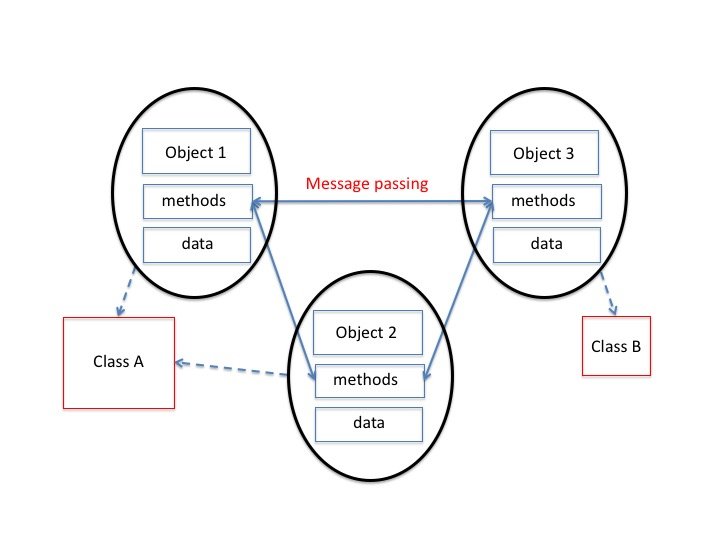
\includegraphics[width=1.2\textwidth]{../../shared/oop_building_blocks.jpg} 
%\end{center} 

  \end{column}
  \begin{column}{0.48\textwidth}
\scriptsize{
    \begin{itemize}
        \item A \textbf{class} is a set of properties and related procedures which access/modify those properties.
        \item \textbf{Objects} are individual instances of classes.
        \begin{itemize}
        \item \scriptsize{Behavior of objects is expressed in terms of methods which are the class procedures. Methods have privileged access to object state.}
        \item \scriptsize{Method invocation may look different than regular procedure calls.}
        \end{itemize}
        \item Within a program, objects interact with each other by sending messages (i.e. invoking methods)
    \end{itemize}
 }
  \end{column}
\end{columns}


\end{frame} 


% --- Slide ---

\begin{frame}{Encapsulation}

\textbf{Encapsulation} is the ability to isolate and hide implementation details within a software subsystem.
\begin{itemize}

  \item Instead of directly accessing items in a data structure, methods are invoked to retrieve/modify. 
  \item If implementation details change, access methods are updated and client code remains unchanged.
  \item E.g.
  \begin{itemize}
  \item month = date \% month $\leftarrow$  Assumes "month" field\\
  becomes\\
  month = getMonth(date) $\leftarrow$ Does not assume "month"
  % Remember - the big wins are for complex software with many complex data structures.
 \end{itemize}
  \item Note: Fortran 90 introduced strong encapsulation capabilities with public/private access for module entities.

 \end{itemize}

\end{frame}

% --- Slide ---

\begin{frame}{Inheritance}

\textbf{Inheritance} is a way to form new classes using classes that have already been defined.
\begin{itemize}

  \item Original class is referred to as the \textbf{base} class (or \textbf{parent} class)
  \item New class is referred to as the \textbf{child} class or \textbf{subclass}
  \item Intent is to reuse significant portions of base class.
  \item Inheritance relations always form hierarchical trees.
  % Remember - the big wins are for complex software with many complex data structures.
  \item Fortran 2003 introduces inheritance (keyword: \textbf{extends})
  \item Child class should be usable in any context where the base class is usable.
  %Child class may add additional fields/components
 % Child class may override some methods of the parent class and leave other behaviors unchanged.
  \begin{itemize}
  \item Useful notion: "is-a" relationship categorization:
    \begin{itemize}
    \item frog is-a kind of amphibian
    \item sparse-matrix is-a kind of matrix
    \end{itemize}
  \end{itemize}
  
 \end{itemize}

\end{frame}

% --- Slide

\begin{frame}{Inheritance example} 
Shape class
\begin{center} 
  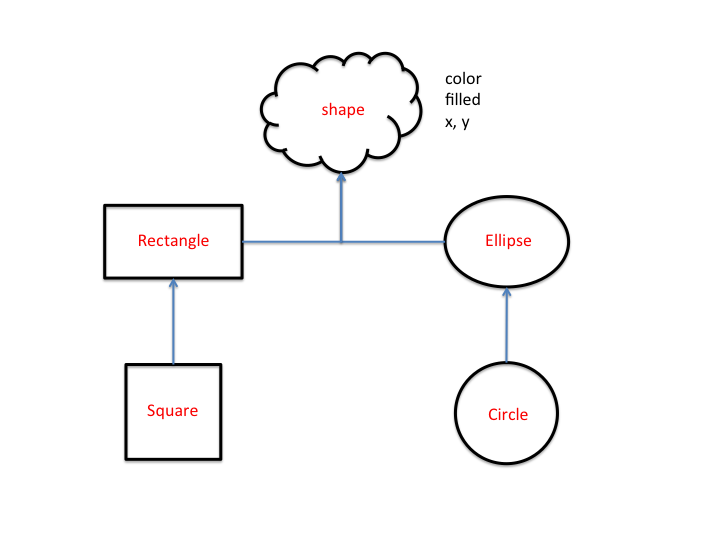
\includegraphics[width=0.9\textwidth]{shapeClass.png} 
\end{center} 

\end{frame} 

% --- Slide ---

\begin{frame}{Function/procedure pointers}

While not strictly an OO concept, function pointers are a major part of the implementation of OO abstractions.
\begin{itemize}

  \item A function pointer is a \emph{data type} that is able to be associated with actual functions/procedures. The association is determined at \emph{run-time}.

  \item Data structure with function pointer can be used to invoke different behavior in different contexts by associating with different actual functions.
  \item Introduced in Fortran 2003
  
 \end{itemize}

\end{frame}



% --- Slide ---

\begin{frame}{Polymorphism}

\textbf{Polymorphism} is the capability of treating objects of a subclass as though they were members of the parent class.
\begin{itemize}

  \item A \textbf{polymorphic variable} is one whose actual type is not known at compile time.
    \begin{itemize}
    \item Run-time environment calls the appropriate methods on depending on actual type (or \textbf{dynamic} type)
    \item Implemented with \textbf{dynamic binding} (usually function pointers)
    \end{itemize}

  \item Polymorphism and inheritance are distinct aspects but are typically applied together for maximum impact.
  \item E.g. polymorphic variable myShape of class ?Shape? will compute the compute area/perimeter according to type set at run time.
  
 \end{itemize}

\end{frame}

% --- Slide ---

\begin{frame}{Advantages of Polymorphism}

\textbf{Polymorphism} is the capability of treating objects of a subclass as though they were members of the parent class.
\begin{itemize}

  \item \emph{Generic programming} - high level algorithms are written in terms of the base class. Do not need to write variants for each subclass.
      \begin{itemize}
    \item E.g. an algorithm working with linear equations can be written in terms of methods for generic matrices, while the specific operations (factor(), solve()) are implemented differently for the subclasses (Dense, Sparse, Banded)
    \end{itemize}

  \item Allows customization \textbf{without} violating encapsulation.
      \begin{itemize}
    \item Extension does not require access to source of the base-class.
    \end{itemize}
  
 \end{itemize}

\end{frame}

% --- Slide ---

\begin{frame}{Aside on Overloading}

AKA \textbf{ad-hoc} polymorphism.
\begin{itemize}

  \item Ability to use the same name for multiple procedures.
    \begin{itemize}
    \item Actual procedure used is determined by type of arguments.
    \end{itemize}

  \item Not based upon any type hierarchy.
    \begin{itemize}
    \item No reuse is possible - each type must have a full implementation of the overloaded procedure.
    \end{itemize}
 
   \item Introduced in Fortran 90 with interface blocks.
 
 \end{itemize}

\end{frame}

% --- Slide ---

\begin{frame}{Templates}

AKA \textbf{Parametric Polymorphism}.
\begin{itemize}

  \item Some languages support the ability to declare multiple similar classes simultaneously.
    \begin{itemize}
    \item Routines using the type then specify which case to use.
    \end{itemize}

  \item Fortran 2003 introduces a limited form.
    \begin{itemize}
    \item Derived types can be parameterized for ?kinds? and sizes.
    \item Cannot parameterize integers and reals simultaneously.
    \end{itemize}
  
 \end{itemize}

\end{frame}

% --- Slide ---

\begin{frame}{OOP and Model Infrastructure}

The clearest case for OOP in scientific models is in the "infrastructure" which manages the various model abstractions.
\begin{itemize}

  \item Infrastructure includes
    \begin{itemize}
    \item I/O
    \item Computational grid
    \item Loop constructs
    \item Domain decomposition
    \item Calendars/clocks
    \end{itemize}

  \item Common infrastructure issues among various Earth system models led to the creation of the ESMF\footnote{Earth System Modeling Framework}. While not truly OO, ESMF is strongly encapsulated and has an object based look-and-feel.
  
 \end{itemize}

\end{frame}


% --- Slide ---

\begin{frame}{Examples}

\begin{itemize}

  \item Air parcel trajectory code
  \begin{itemize}
  \item Needs to support multiple vector fields
  \item Needs to support multiple integration schemes   
  \end{itemize}
  
  \item Multiple Computational Grids

  \begin{itemize}
  \item E.g. for coupled Earth systems we might have
  \begin{itemize}
  \item Lat-Lon (Arakawa A, B, C, D)
  \item Cubed-Sphere
  \item Icosahedral
   \end{itemize}
   \item Some subsystems can "work" with any grid, while others are dependent on specific representations.
   \item Coupling can require custom interpolations between grids.
   \item Can we provide a software layer that supports various grid-specific operations while hiding the details from the layers that don't really care which grid is being used?
   % Domain-decomposition, halo-fill
   % I/O operations
   \end{itemize}

 \end{itemize}

\end{frame}


% --- Slide

\begin{frame}[fragile]
\frametitle{Conclusion}

\FontCcolumn

\begin{itemize}
\item F2003 includes a solid support of object orientation.
\item Provides opportunities to adopt newer technologies and modernize current earth science models.
\item There is already a F2008 standard, but enhancements are "minor" (submodules, co-arrays)...and it may take a lot longer for compilers to adopt the standard.
\end{itemize}

\bigskip
References:
\begin{itemize}
\item John Reid, "The new features of Fortran 2003, ACM SIGPLAN Fortran Forum 96", 10 (2007)
\item http://www.nag.com/nagware/NP/doc/nag\_f2003.pdf
\item http://www.pgroup.com/doc/pgifortref.pdf
\end{itemize}
\end{frame}

\end{document}